\subsection{base\_sum}

BaseSumGate is used to constrain the input to be composed of limbs which are arranged in little-endian. There are two kinds of constraints:

For each limb, limb is in range [0, base):
\[\sum_{i=0}^{base}(limb_i - i) = 0\]

Input is composed of limbs:
\[input = \sum_{i=0}^{n-1} limb_{n-1-i} * base^i\]

\begin{figure}[!h]
    \centering
    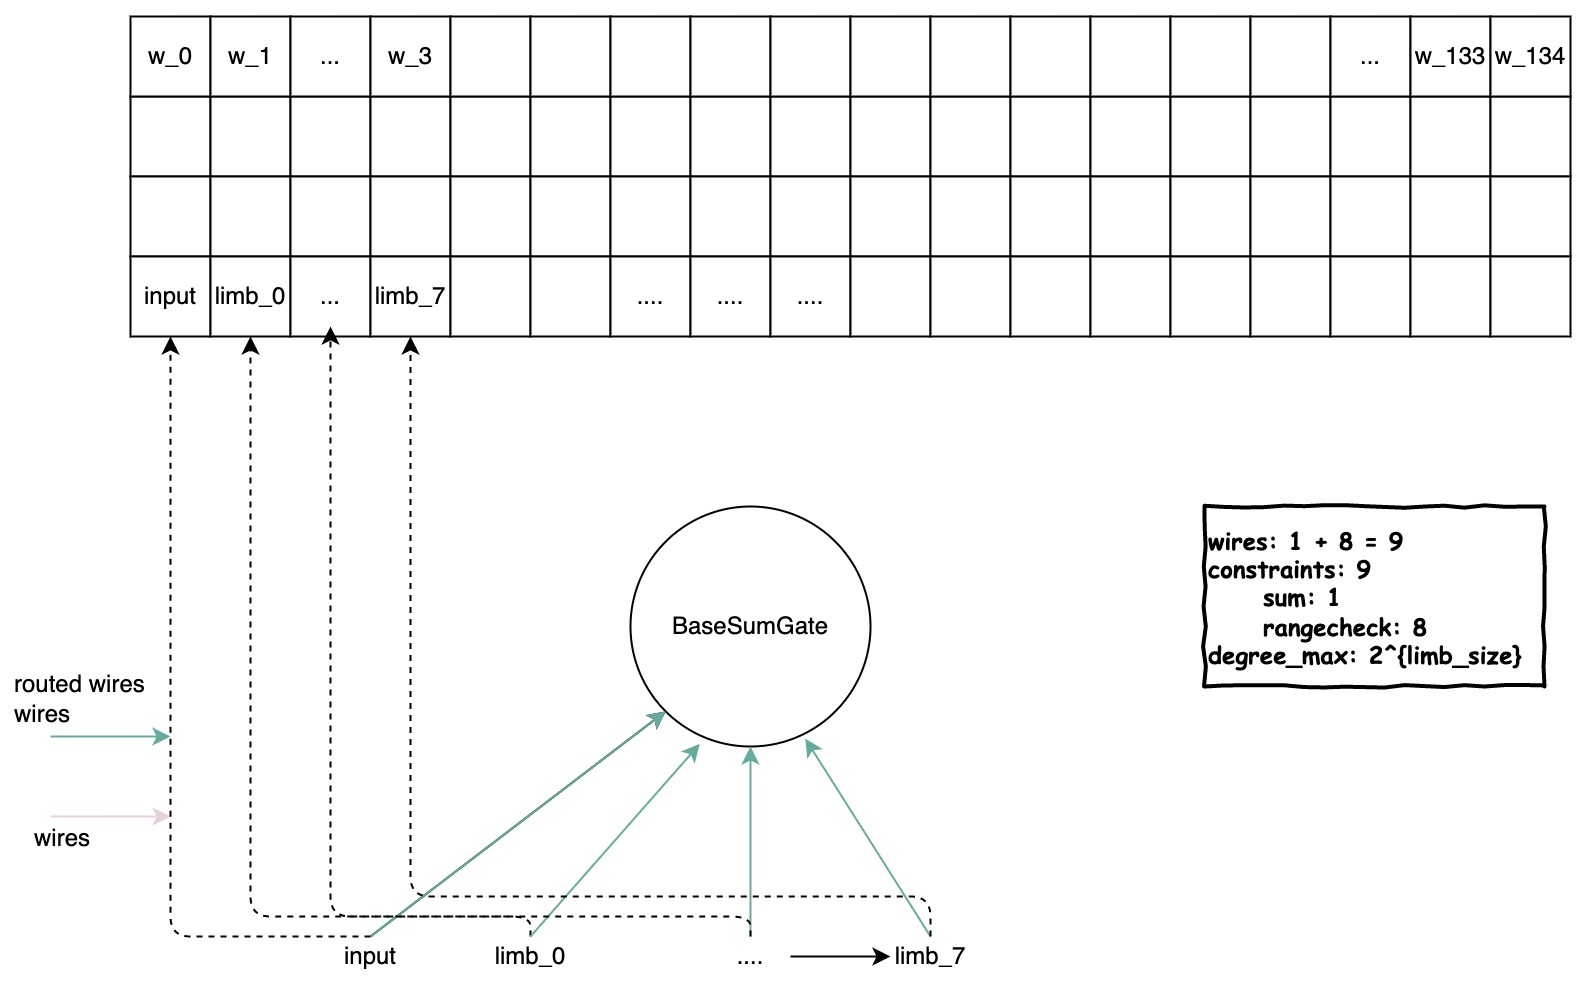
\includegraphics[width=0.8\textwidth]{gates/base_sum.jpeg}
    \caption{BaseSumGate}
    \label{fig:base-sum}
\end{figure}